\documentclass{article}
\usepackage[utf8]{inputenc}
\usepackage{longtable}
\usepackage{authblk}
\usepackage{adjustbox}
\usepackage{natbib}

\title{CARACTERIZACIÓN DE LOS INDICES DE DESARROLLO HUMANO EN COLOMBIA}
% autores
\renewcommand\Authand{, y }
\author[1]{\normalsize Carolina Barreto Naranjo}
\author[2]{\normalsize Andrea Calderon Corredor}
\author[3]{\normalsize Andrea Blanco Zarta}

\affil[1,2,3]{\small  Facultad de Ingeniería,Universidad de los Andes\\
\texttt{{c.barreto805,a.calderon,a.blanco}@uniandes.edu.co}}
\affil[1,2,3]{\small Herramientas Computacionales para la Investigacion\\}

\date{29 de Junio de 2018}

\usepackage{Sweave}
\begin{document}
\Sconcordance{concordance:matriz.tex:matriz.Rnw:%
1 22 1 1 0 37 1}


\maketitle


\begin{abstract}
En este trabajo se hace un análisis de la evolución del IDH como indicador social. Primero se realiza una discusión sobre la importancia de colocar en la agenda social al IDH. Posteriormente se presentan los elementos que componente el IDH. Por último se analizan los indicadores del IDH tanto a nivel global como para México. La desigualdad existe desde los primeros hombres, esta se debe medir y se debería de crear un consenso sobre la forma de medirla y de compararla entre los distintos países, estados y entidades de distinta índole. Al hablar de la igualdad, se debe de tomar en cuenta desde qué “ángulo” estamos viendo la situación, desde la perspectiva del utilitarismo o no. También influye el ámbito de estudio de las igualdades, por ejemplo, la igualdad en salud implica una serie de igualdades asociadas como son la igualdad de inclusión, de asistencia, de educación, de libertad, etc. Amartya Sen preguntó “igualdad ¿de qué?” pues en no pocas ocasiones al pedir la igualdad respecto a “A” se perjudica a otro tipo de igualdad respecto a “B”. El Índice de Desarrollo Humano(IDH), es un índice compuesto del índice de salud, índice de educación y el índice de ingresos. 
\end{abstract}

\section*{Introducción}

El Índice de Desarrollo humano (IDH) es un indicador creado por el Programa de las Naciones Unidas para el Desarrollo (PNUD) con el fin de determinar el nivel de desarrollo que tienen los países del mundo.  Fue ideado con el objetivo de conocer, no sólo los ingresos económicos de las personas en un país, sino también para evaluar si el país aporta a sus ciudadanos un ambiente donde puedan desarrollar mejor o peor su proyecto y condiciones de vida.  Para esto, el IDH tiene en cuenta tres variables:

1) Esperanza de vida al nacer. Analiza el promedio de edad de las personas fallecidas en un año.

2) Educación. Recoge el nivel de alfabetización adulta y el nivel de estudios alcanzado (primaria, secundaria, estudios superiores)

3) PIB per Cápita (a paridad de poder adquisitivo). Considera el producto interno bruto per cápita y evalúa el acceso a los recursos económicos necesarios para que las personas puedan tener un nivel de vida decente.

El índice IDH aporta valores entre 0 y 1,  siendo 0 la calificación más baja y 1 la más alta. En este sentido, la PNUD clasifica a los países en tres grandes grupos:

Países con Alto desarrollo Humano (“High Human Development”).  Tienen un IDH mayor de 0,80. 

Países con Medio desarrollo Humano (“Medium Human Development”). Tienen un IDH entre 0,50 y 0,80.

Países con Bajo desarrollo Humano (“Low Human Development”). Tienen un IDH menor de 0,50.

La principal amenaza al progreso en América Latina y El Caribe es la recaída de millones de hogares en la pobreza, pero la ralentización económica no es la única culpable de tal regresión. El informe presenta recomendaciones para que los países de la región -incluido Colombia- impidan retrocesos y siga avanzando en lo social, económico y ambiental, con políticas públicas de nueva generación, en línea con los Objetivos de Desarrollo Sostenible (ODS).

Así lo explicó el autor principal, George Gray Molina, jefe de Economía del Bureau del PNUD para América Latina y el Caribe, quien presentó la investigación a funcionarios del Gobierno colombiano, la sociedad civil, el sector privado, entre otros, que asistieron al evento organizado por PNUD Colombia.
El informe, titulado “Progreso Multidimensional: bienestar más allá del ingreso”, propone un concepto de desarrollo que tiene como eje central la riqueza de la vida humana y el bienestar, considerando que el progreso medido únicamente a través del ingreso monetario no ha servido para el desarrollo integral de las personas en la región. 

En este panorama, el informe plantea considerar las distintas variables que inciden en el desarrollo como: la mejora del acceso y la calidad de los servicios básicos, un sistema de cuidado, el cierre de brechas históricas de género, raza y etnia y la protección del medio ambiente. La idea principal en la que se ampara el informe es que “nada que disminuya los derechos de las personas y comunidades, o que amenace la sostenibilidad ambiental puede ser considerado progreso”. 

En este sentido, el PNUD enfatiza que el bienestar de la gente es “más que ingreso”, y llama a que los líderes y decisores de la región se centren en el logro de un “progreso multidimensional”.


Comencemos viendo que hay en la sección \ref{univariada} en la página \pageref{univariada}.

\clearpage


\section{Exploración Univariada}\label{univariada}




Teniendo en cuenta queel estudio se hizo para los 32 departamentos de Colombia

% Table created by stargazer v.5.2.2 by Marek Hlavac, Harvard University. E-mail: hlavac at fas.harvard.edu
% Date and time: vie., jun. 29, 2018 - 7:22:42 p.m.
\begin{table}[!htbp] \centering 
  \caption{Medidas estadísticas} 
  \label{stats} 
\begin{tabular}{@{\extracolsep{5pt}}lccccc} 
\\[-1.8ex]\hline 
\hline \\[-1.8ex] 
Statistic & \multicolumn{1}{c}{Mean} & \multicolumn{1}{c}{Median} & \multicolumn{1}{c}{St. Dev.} & \multicolumn{1}{c}{Min} & \multicolumn{1}{c}{Max} \\ 
\hline \\[-1.8ex] 
IDH & 0.802 & 0.804 & 0.042 & 0.691 & 0.879 \\ 
Poblacion.Cabecera & 1,196,730.000 & 717,197 & 1,982,287.000 & 13,090 & 10,070,801 \\ 
Poblacion.Resto & 360,590.300 & 268,111.5 & 331,887.600 & 21,926 & 1,428,858 \\ 
Poblacion.Total & 1,557,320.000 & 1,028,429 & 2,202,522.000 & 43,446 & 10,985,285 \\ 
\hline \\[-1.8ex] 
\end{tabular} 
\end{table} \centering




\begin{figure}[h]
\centering
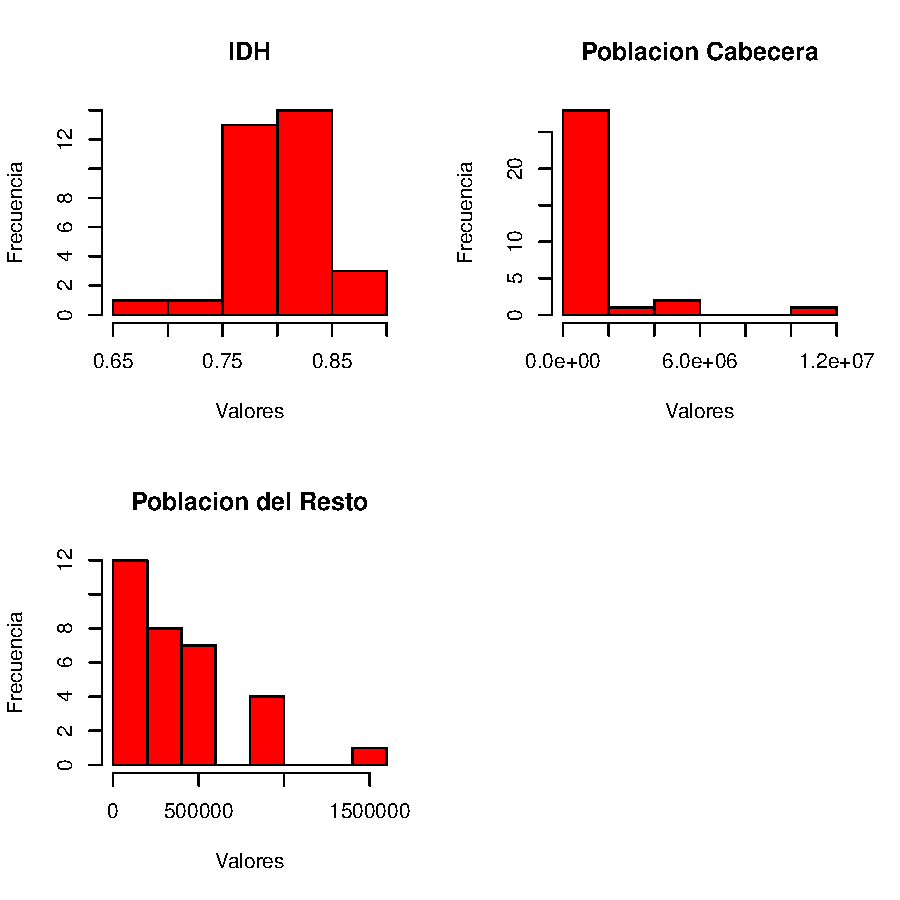
\includegraphics{univariada-hist}
\caption{Distribuci?n de Indicadores}
\label{hist}
\end{figure}

Si quieren normalizar dado el sesgo de las poblaciones, se tranforma con logaritmo en case 10 y quedaria asi:

\begin{figure}[h]
\centering
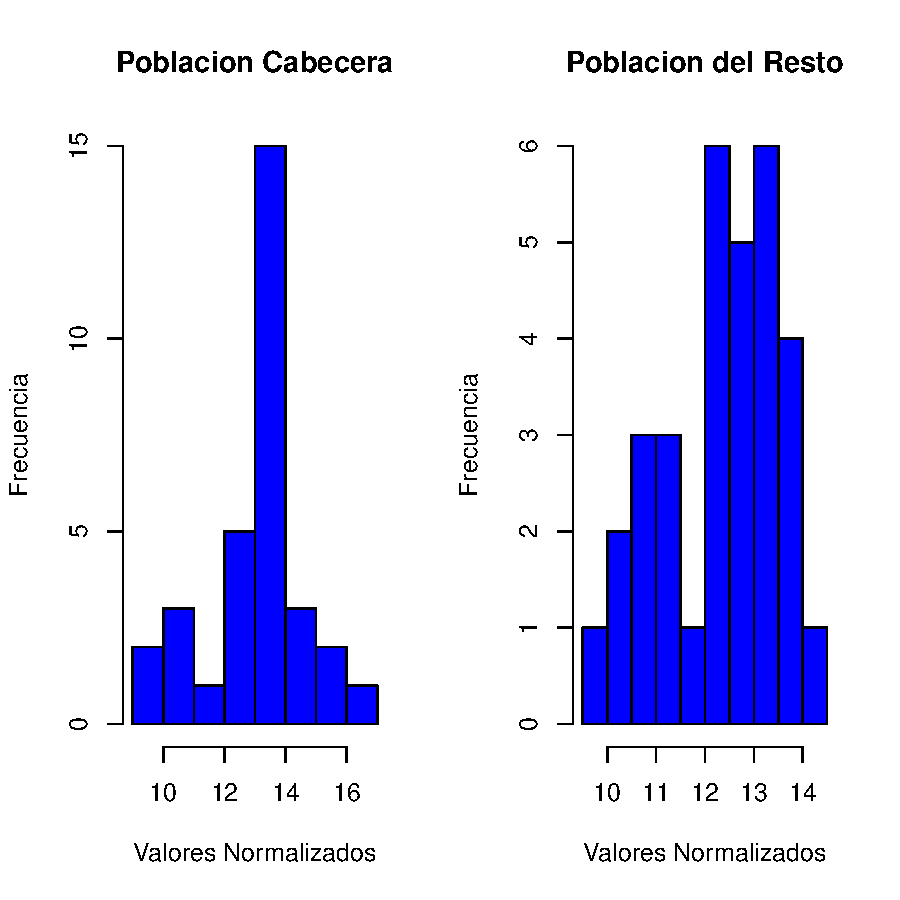
\includegraphics{univariada-hist1}
\caption{Distribuci?n de Indicadores de Poblaciones Normalizado}
\label{hist1}
\end{figure}

\endinput




\bibliographystyle{apalike}
\renewcommand{\refname}{Bibliography}
\bibliography{Colombia}

\end{document}
